\documentclass[10pt]{beamer}

\usetheme{metropolis}
\usepackage{appendixnumberbeamer}

\usepackage{booktabs}
\usepackage[scale=2]{ccicons}
\usepackage{graphicx}
\usepackage{hyperref}
\usepackage{circuitikz}
\usepackage{pdflscape}
\usepackage{smartdiagram}

\usepackage{color}
\usepackage{listings}

\lstset{
	basicstyle=\footnotesize\ttfamily,
    keepspaces=true,
    showstringspaces=false,
    language=PHP,
    commentstyle=\ttfamily,
}

\usepackage[OT4]{polski}
\usepackage[utf8]{inputenc}

\usepackage{pgfplots}
\usepgfplotslibrary{dateplot}

\usepackage{xspace}
\newcommand{\themename}{\textbf{\textsc{metropolis}}\xspace}

\setbeamertemplate{frame footer}{}
\setbeamertemplate{frame numbering}{}

\usetikzlibrary{shapes,arrows}

\tikzstyle{decision} = [diamond, draw, fill=blue!20, 
    text width=4.5em, text badly centered, node distance=3cm, inner sep=0pt]
\tikzstyle{block} = [rectangle, draw, fill=blue!20, 
    text width=5em, text centered, rounded corners, minimum height=4em]
\tikzstyle{line} = [draw, -latex']
\tikzstyle{cloud} = [draw, ellipse,fill=red!20, node distance=3cm,
    minimum height=2em]


\title{Zasady SOLID}

\subtitle{Projektowanie i programowanie systemów internetowych I}
\author{mgr inż. Krzysztof Rewak}
\date{\today}
\institute{Wydział Nauk Technicznych i Ekonomicznych \\ Państwowa Wyższa Szkoła Zawodowa im. Witelona w Legnicy}

\begin{document}

\maketitle

\begin{frame}{Plan prezentacji}
  \setbeamertemplate{section in toc}[sections numbered]
  \tableofcontents[hideallsubsections]
\end{frame}


\begin{frame}{SOLID}
	\textbf{SOLID} to mnemoniczny akronim zaproponowany przez amerykańskiego programistę Roberta C. Martina.
\end{frame}

\begin{frame}{SOLID}
	Dotyczy on pięciu podstawowych zasad tworzenia oprogramowania. Stosowanie się do nich powinno zwiększyć jakość tworzonego kodu pod względem jego czytelności, elastyczności i zdatności do szeroko rozumianego utrzymywania.
\end{frame}

\begin{frame}{SOLID}
	W programistycznym świecie zasady SOLID to podstawa, zarówno przy projektowaniu i implementacji systemów informatycznych, jak i przy rekrutacji nowych członków zespołu.
\end{frame}

\begin{frame}{SOLID}
	Część z tych zasad bywa czasami natualnie odkrywana przez mniej doświadczonych programistów. Warto jednak wykorzystać mnemonikę Martina, aby w przyszłości móc bezpośrednio odpowiedzieć na pytania innych programistów.
\end{frame}

\section{S}

\begin{frame}{Zasada pojedynczej odpowiedzialności}
	\textbf{S} (lub \textbf{SRP}) to \emph{single responsibility principle}, czyli zasada pojedynczej odpowiedzialności.
\end{frame}

\begin{frame}{Zasada pojedynczej odpowiedzialności}
	Najprawdopodobniej najprostsza do samodzielnego wywnioskowania, zasada jednej odpowiedzialności mówi, że jedna klasa powinna realizować tylko jeden cel.
\end{frame}

\begin{frame}{Zasada pojedynczej odpowiedzialności}
	W \emph{Czystym kodzie} Martin sugeruje, że:
	\begin{itemize}
		\item
		\item
	\end{itemize}
\end{frame}

\begin{frame}{Zasada pojedynczej odpowiedzialności}
	W \emph{Czystym kodzie} Martin sugeruje, że:
	\begin{itemize}
		\item klasy powinny być małe,
		\item
	\end{itemize}
\end{frame}

\begin{frame}{Zasada pojedynczej odpowiedzialności}
	W \emph{Czystym kodzie} Martin sugeruje, że:
	\begin{itemize}
		\item klasy powinny być małe,
		\item klasy powinny być mniejsze niż są.
	\end{itemize}
\end{frame}

\begin{frame}{Zasada pojedynczej odpowiedzialności}
	Funkcje można mierzyć licząc liczbę linii kodu, z których się składają. Im więcej, tym zazwyczaj gorzej.
	
	Klasy natomiast można zmierzyć za pomoca metryki tzw. odpowiedzialności. 
\end{frame}

\begin{frame}{Zasada pojedynczej odpowiedzialności}
	Wyobraźmy sobie klasę implementującą dany interfejs \texttt{UserService}:
\end{frame}

\begin{frame}{Zasada pojedynczej odpowiedzialności}
	\begin{figure}
		\centering
		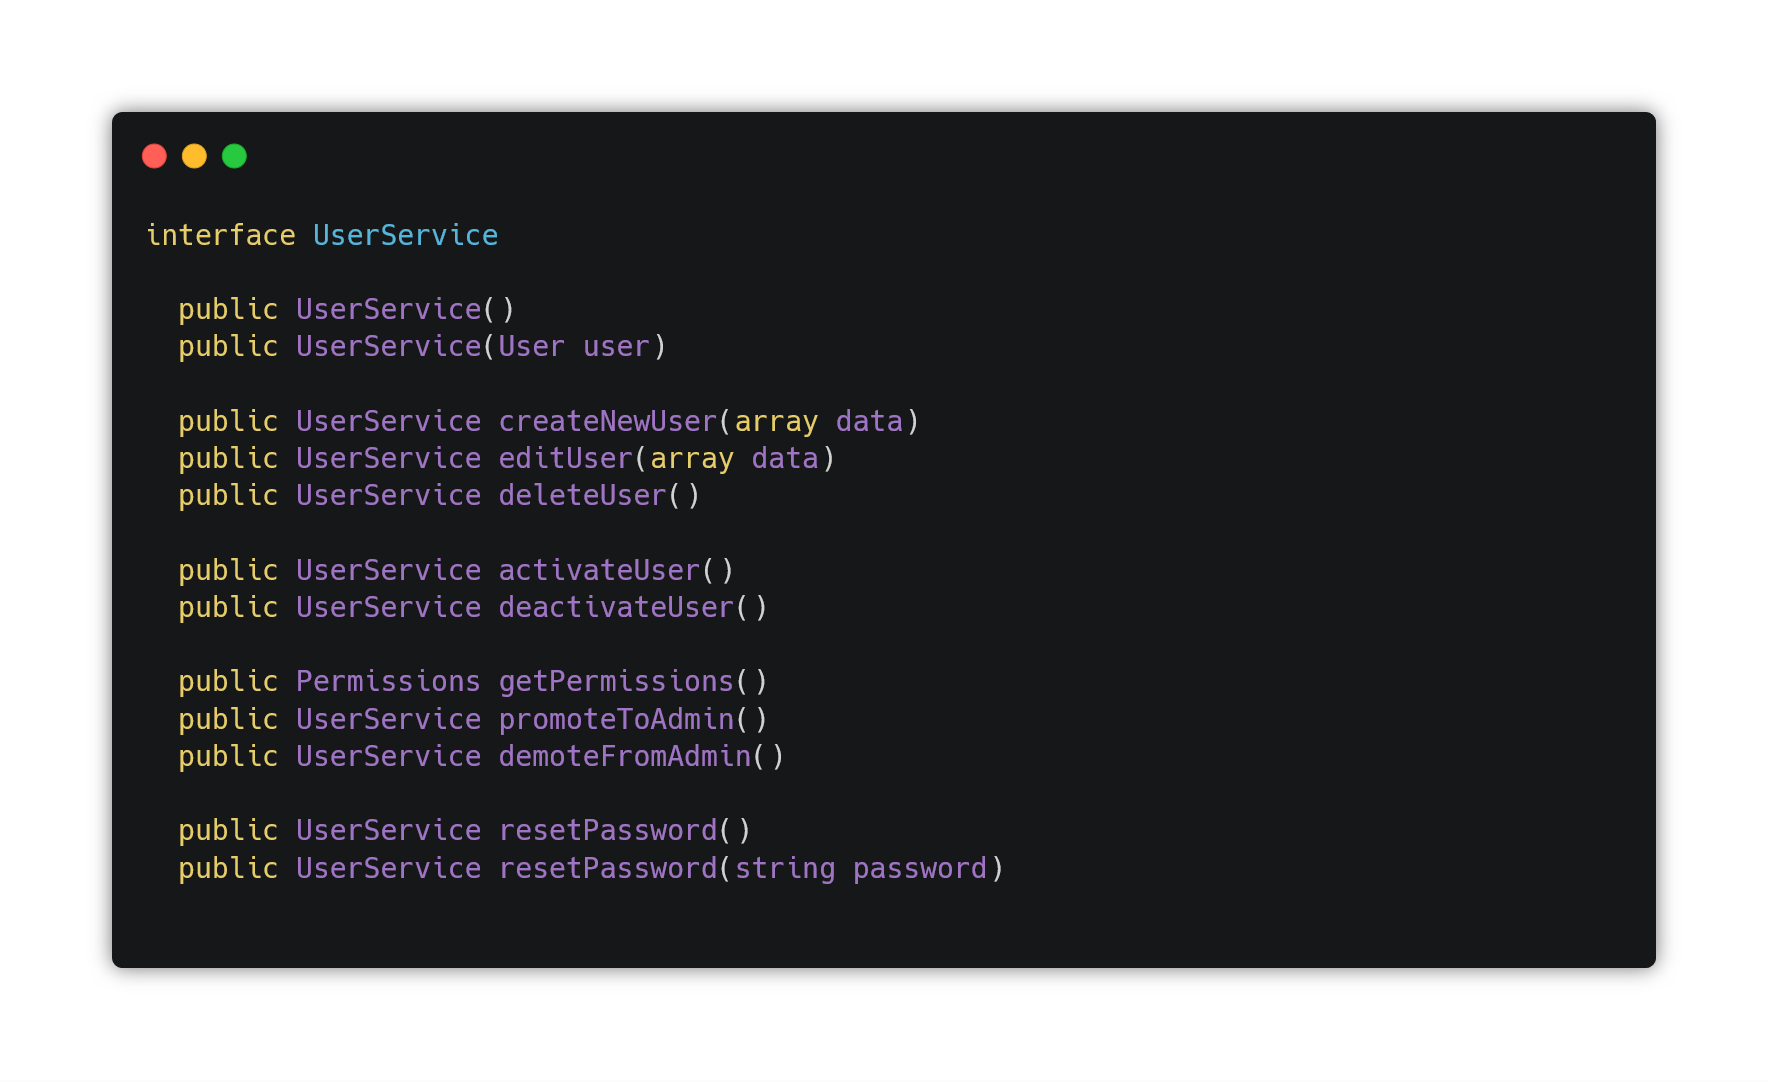
\includegraphics[width=\textwidth]{userservice.png}
	\end{figure}
\end{frame}

\begin{frame}{Zasada pojedynczej odpowiedzialności}
	Jaki jest zakres odpowiedzialności tej klasy?
	
	Co by się stało, gdybyśmy się umówili na odrzucenie nic nie mówiących nazw takich jak \texttt{UserService} i nazywali klasy zgodnie z ich odpowiedzialnością?
\end{frame}

\begin{frame}{Zasada pojedynczej odpowiedzialności (ałć!)}
	\begin{figure}
		\centering
		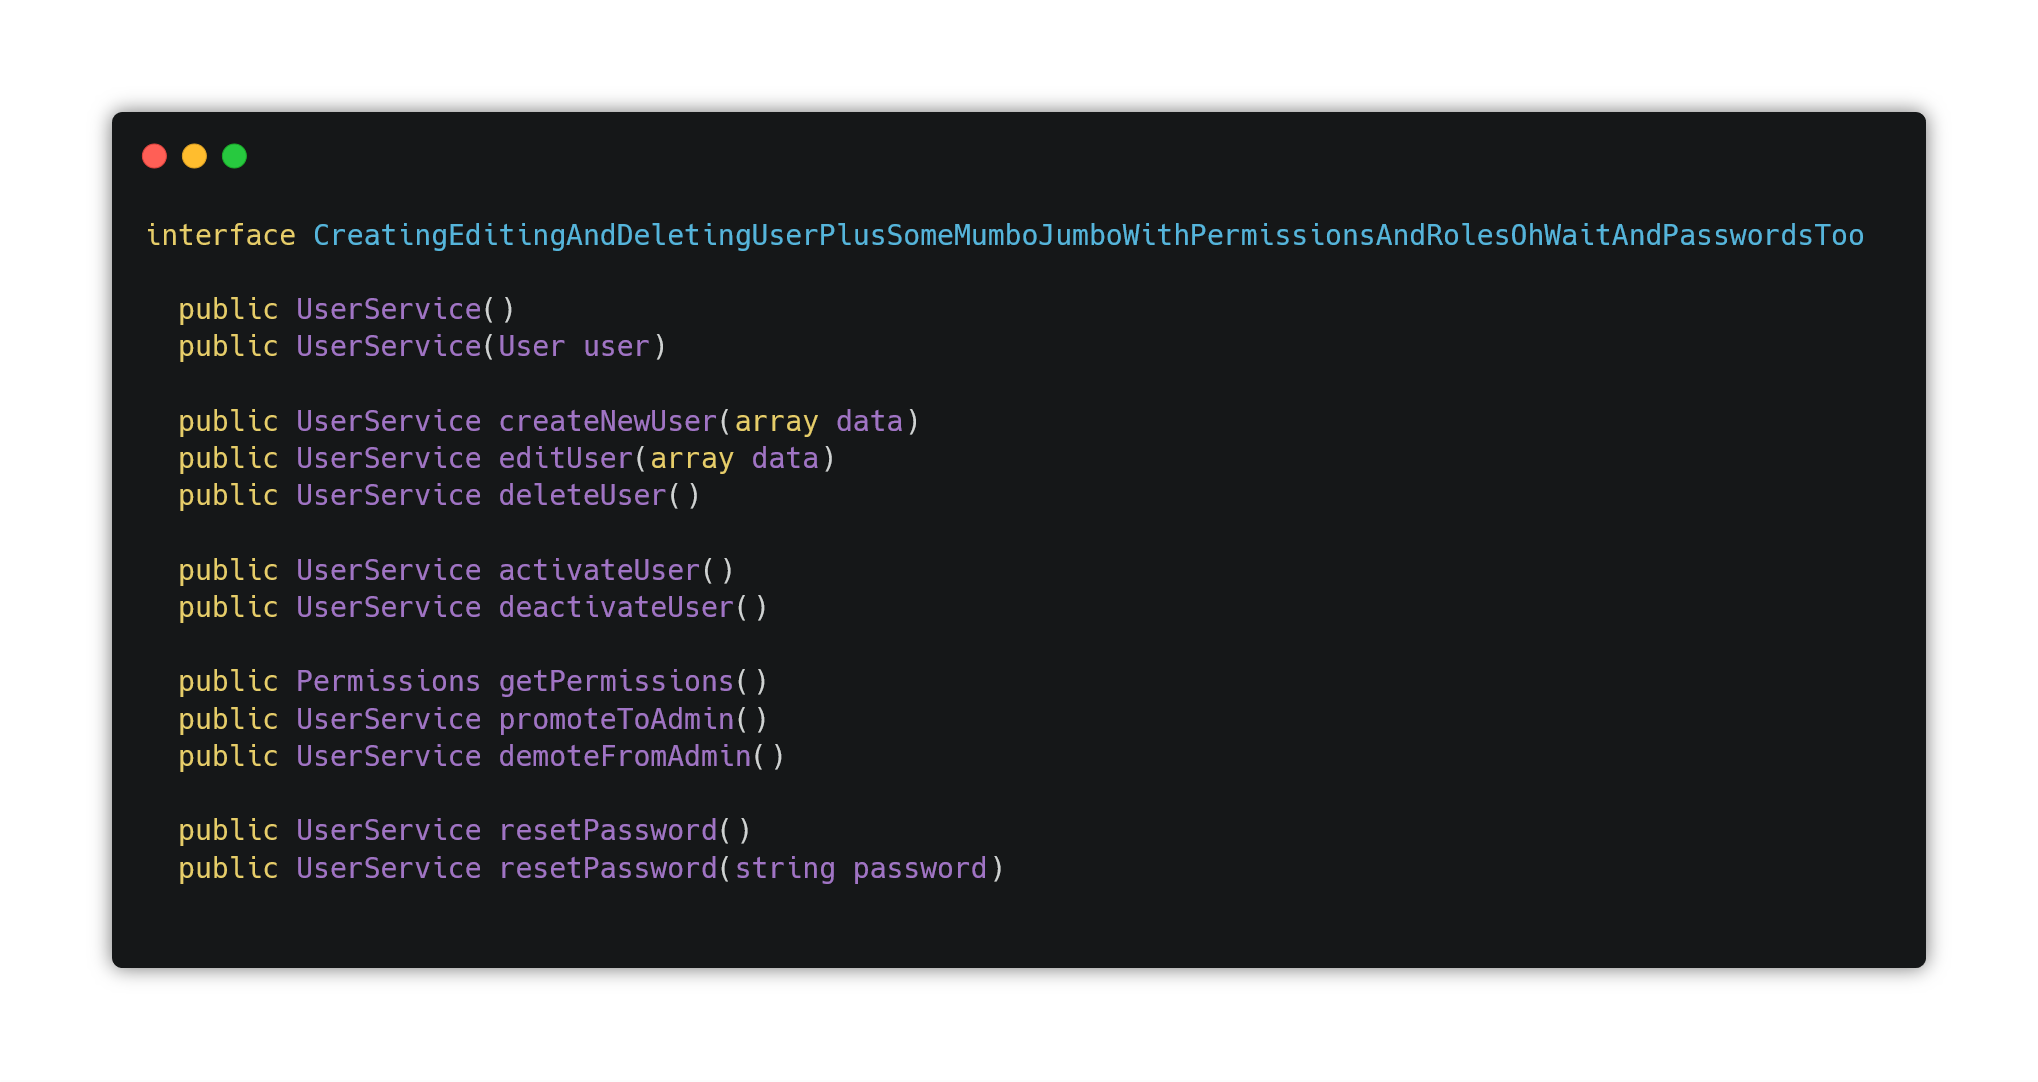
\includegraphics[width=\textwidth]{looongname.png}
	\end{figure}
\end{frame}

\begin{frame}{Zasada pojedynczej odpowiedzialności}
	Idea stojąca za SRP zakłada, że klasa powinna mieć tylko jeden \emph{powód do zmiany}. Czyż poniższa klasa nie wygląda lepiej?
	
	\begin{figure}
		\centering
		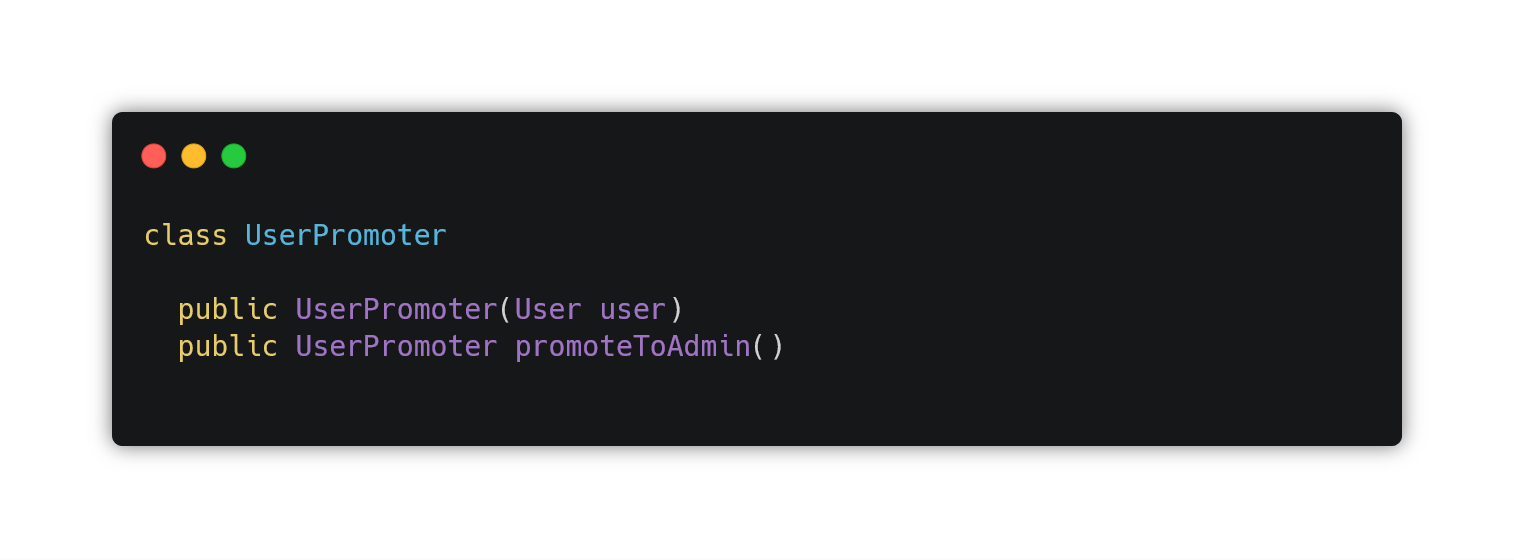
\includegraphics[width=\textwidth]{userpromoter.png}
	\end{figure}
\end{frame}

\begin{frame}{Zasada pojedynczej odpowiedzialności}
	Wygląda na to, że SRP jest faktycznie proste... jednakże jest również najczęściej łamane. 
	
	Podstawowym powodem takiego (przykrego) stanu jest strach przed zbytnim \emph{napompowaniem} projektu wieloma klasami. Ale czy jednak klasa z czterdziestoma metodami na prawdę jest lepsza od czterdziestu klas z jedną metodą?
\end{frame}

\section{O}

\begin{frame}{Zasada otwarte-zamknięte}
	\textbf{O} (lub \textbf{OCP}) to \emph{open/closed principle}, czyli zasada otwarte-zamknięte.
\end{frame}

\begin{frame}{Zasada otwarte-zamknięte}
	Zgodnie z zasadami klasy powinny być \textbf{otwarte} na rozszerzenia i \textbf{zamknięte} na modyfikacje.
\end{frame}

\begin{frame}{Zasada otwarte-zamknięte}
	Co to znaczy?
	
	Chodzi o to, aby w razie potrzeby zmian, istniejący już kod nie był modyfkikowany.
\end{frame}

\begin{frame}{Zasada otwarte-zamknięte (ałć!)}
	\begin{figure} \centering
		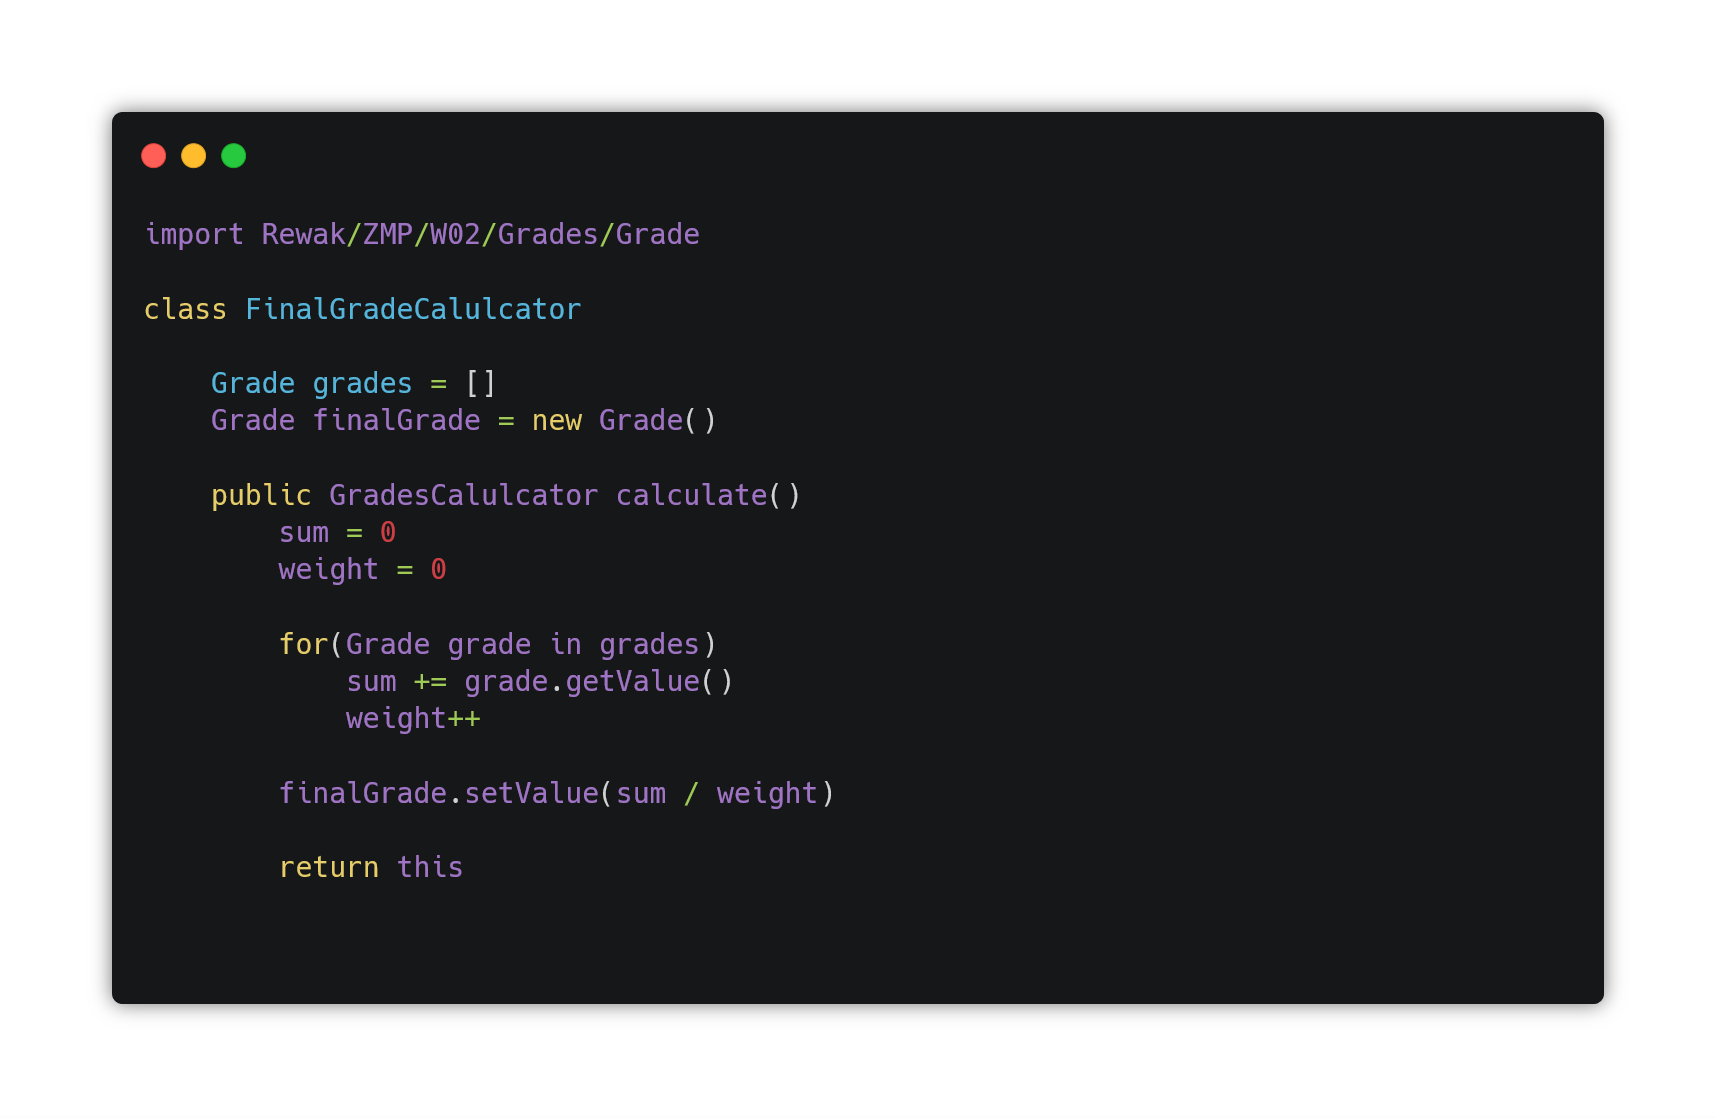
\includegraphics[width=\textwidth]{grades.png}
	\end{figure}
\end{frame}

\begin{frame}{Zasada otwarte-zamknięte}
	Kod z poprzedniego slajdu liczy średnią ocen studenta z podanych ocen cząstkowych. Nic trudnego.
	
	Czy została zachowana zasada otwarte/zamknięte? Co się stanie jeżeli będziemy chcieli dodać do tego wszystkiego ważone oceny?
\end{frame}

\begin{frame}{Zasada otwarte-zamknięte (ałć!)}
	\begin{figure} \centering
		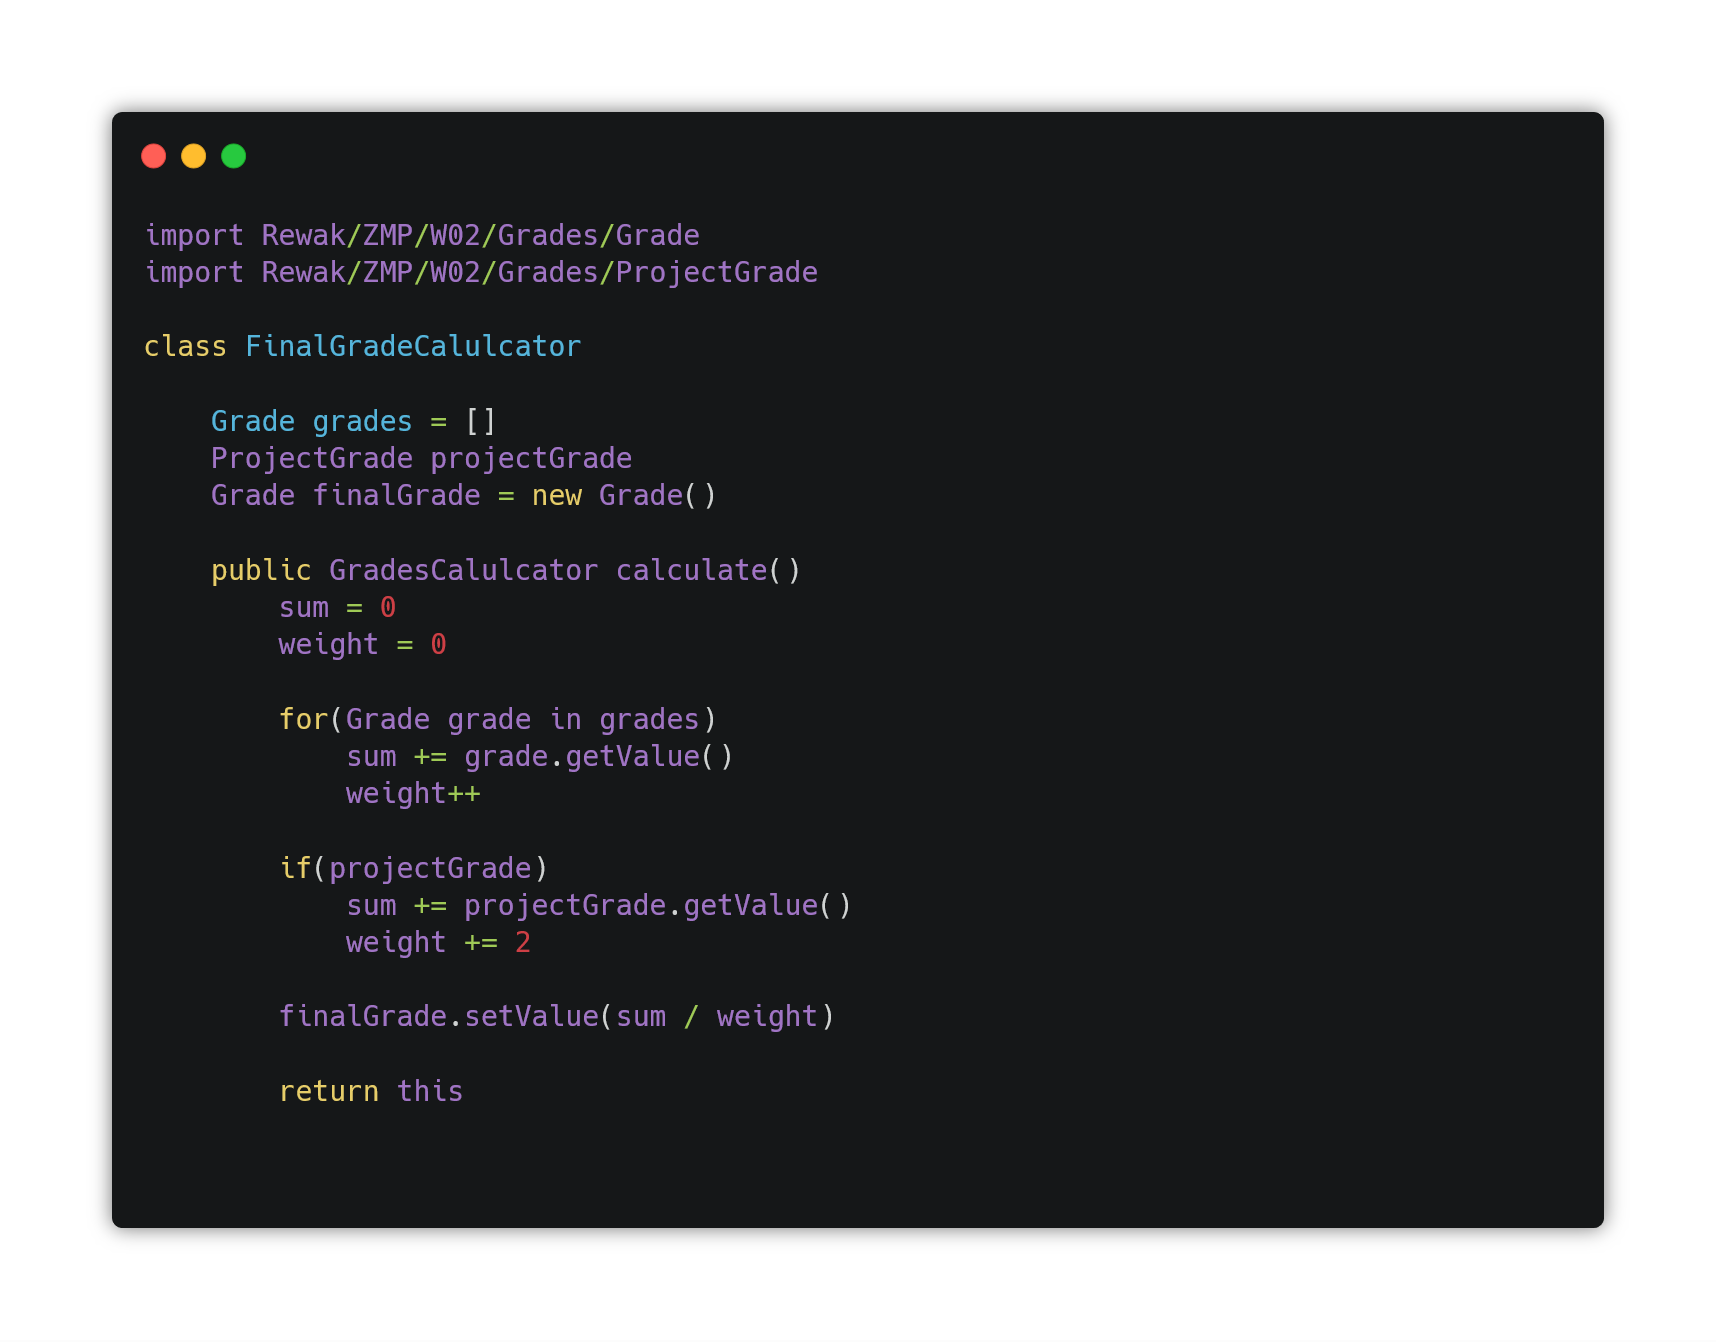
\includegraphics[width=\textwidth]{grades1.png}
	\end{figure}
\end{frame}

\begin{frame}{Zasada otwarte-zamknięte}
	Lipa.
	
	Żeby dodać możliwość ważenia średniej musieliśmy zmienić sposób przeprowadzania obliczeń. A co jeżeli, będziemy mieli więcej rodzajów ocen?
\end{frame}

\begin{frame}{Zasada otwarte-zamknięte}
	\begin{figure} \centering
		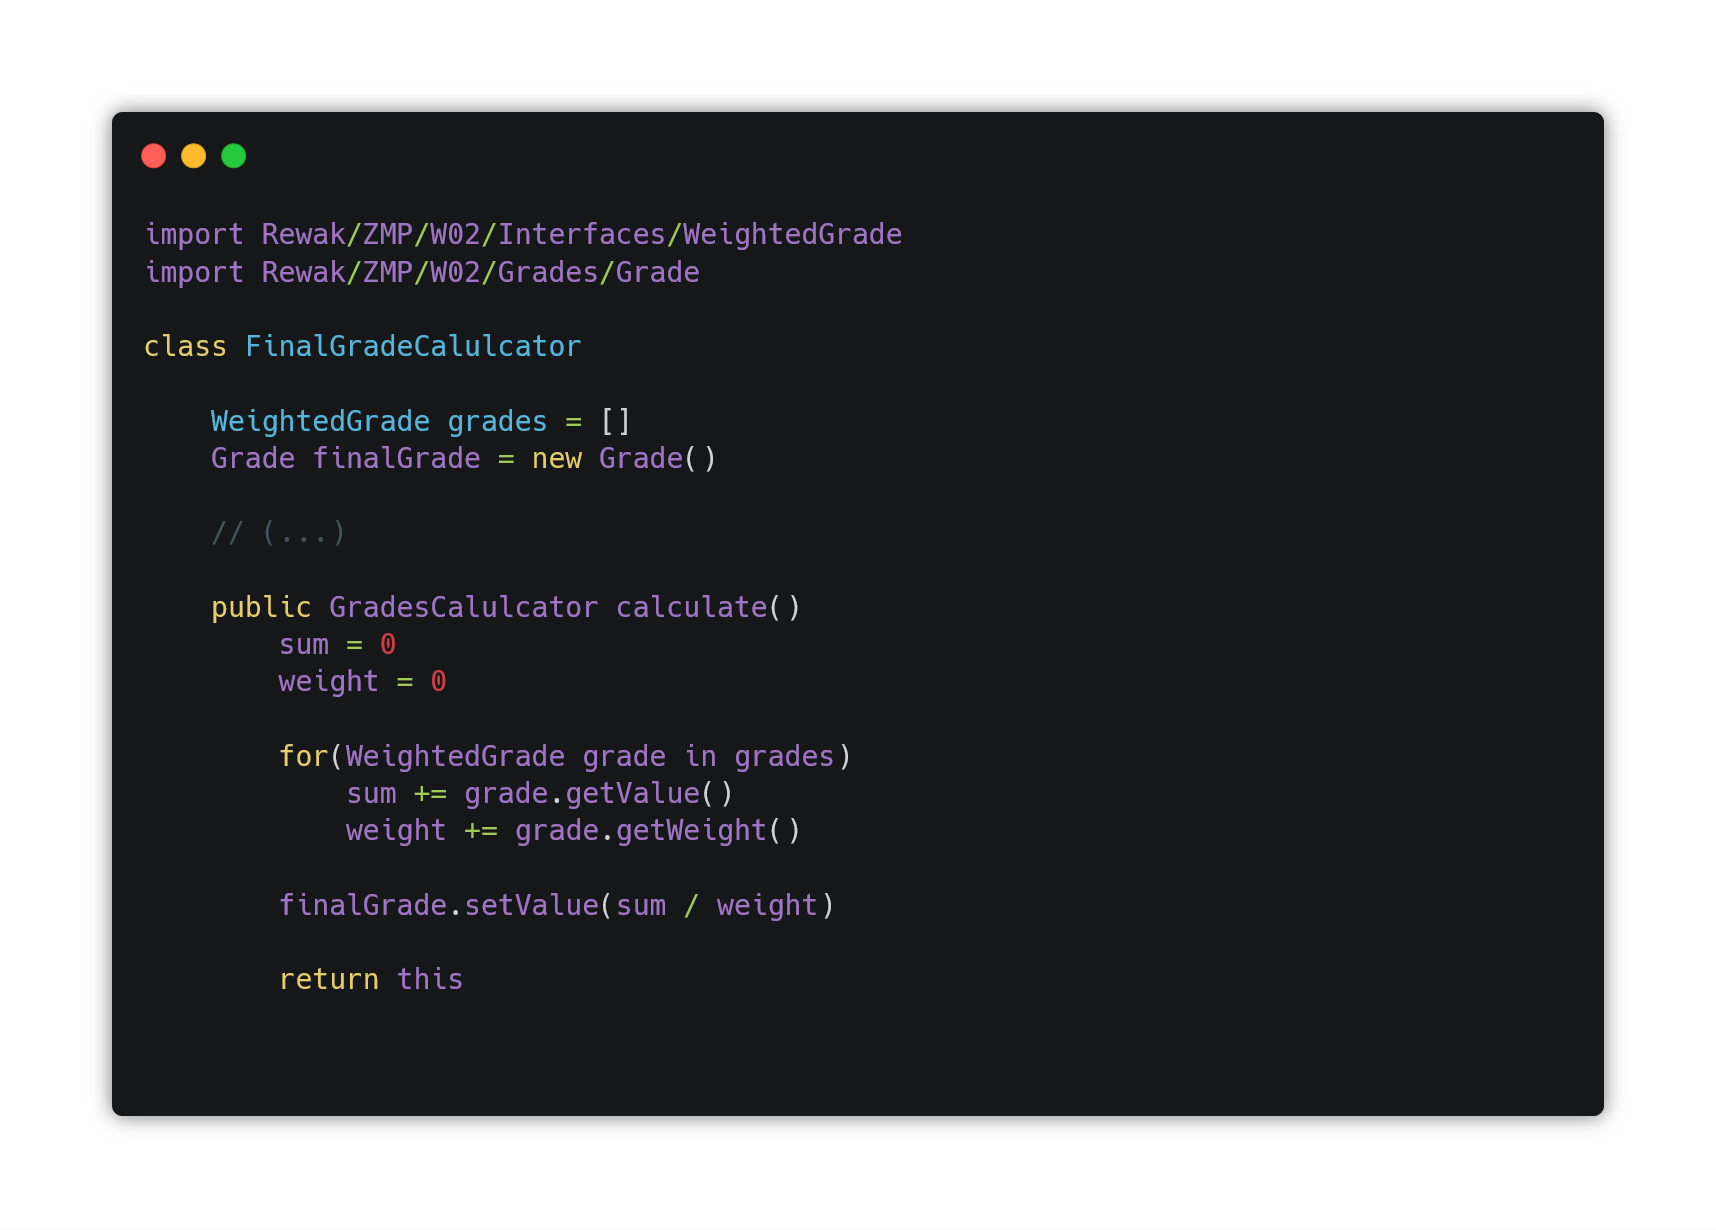
\includegraphics[width=\textwidth]{grades2.png}
	\end{figure}
\end{frame}

\begin{frame}{Zasada otwarte-zamknięte}
	Korzystając z interfejsu możemy uelastycznić nasz serwis.
	
	Czy dana implementacja rozwiąże wszystkie nasze problemy? Oczywiście, że nie.
	
	A czy poprawi jakoś kodu?
\end{frame}

\section{L}

\begin{frame}{Zasada podstawienia Liskov}
	\textbf{L} (lub \textbf{LSP}) to \emph{Liskov substitution principle}, czyli zasada podstawienia Liskov.
\end{frame}

\begin{frame}{Zasada podstawienia Liskov}
	\emph{Funkcje które używają wskaźników lub referencji do klas bazowych, muszą być w stanie używać również obiektów klas dziedziczących po klasach bazowych, bez dokładnej znajomości tych obiektów.}
\end{frame}

\begin{frame}{Zasada podstawienia Liskov}
	Barbara Liskov sformułowała tę zasadę w \emph{Data Abstraction and Hiererchy} w 1987. Z całej piątki SOLID to właśnie LSP brzmi najbardziej skomplikowanie, ale czy na pewno jest trudna do zrozumienia?
\end{frame}

\begin{frame}{Zasada podstawienia Liskov}
	Korzystając z dziedziczenia powinniśmy tak tworzyć nowe klasy, żeby jedynie rozszerzały możliwości rodzica.
	
	Roszerzały, ale nie modyfikowały!
\end{frame}

\begin{frame}{Zasada podstawienia Liskov (ałć!)}
	\begin{figure} \centering
		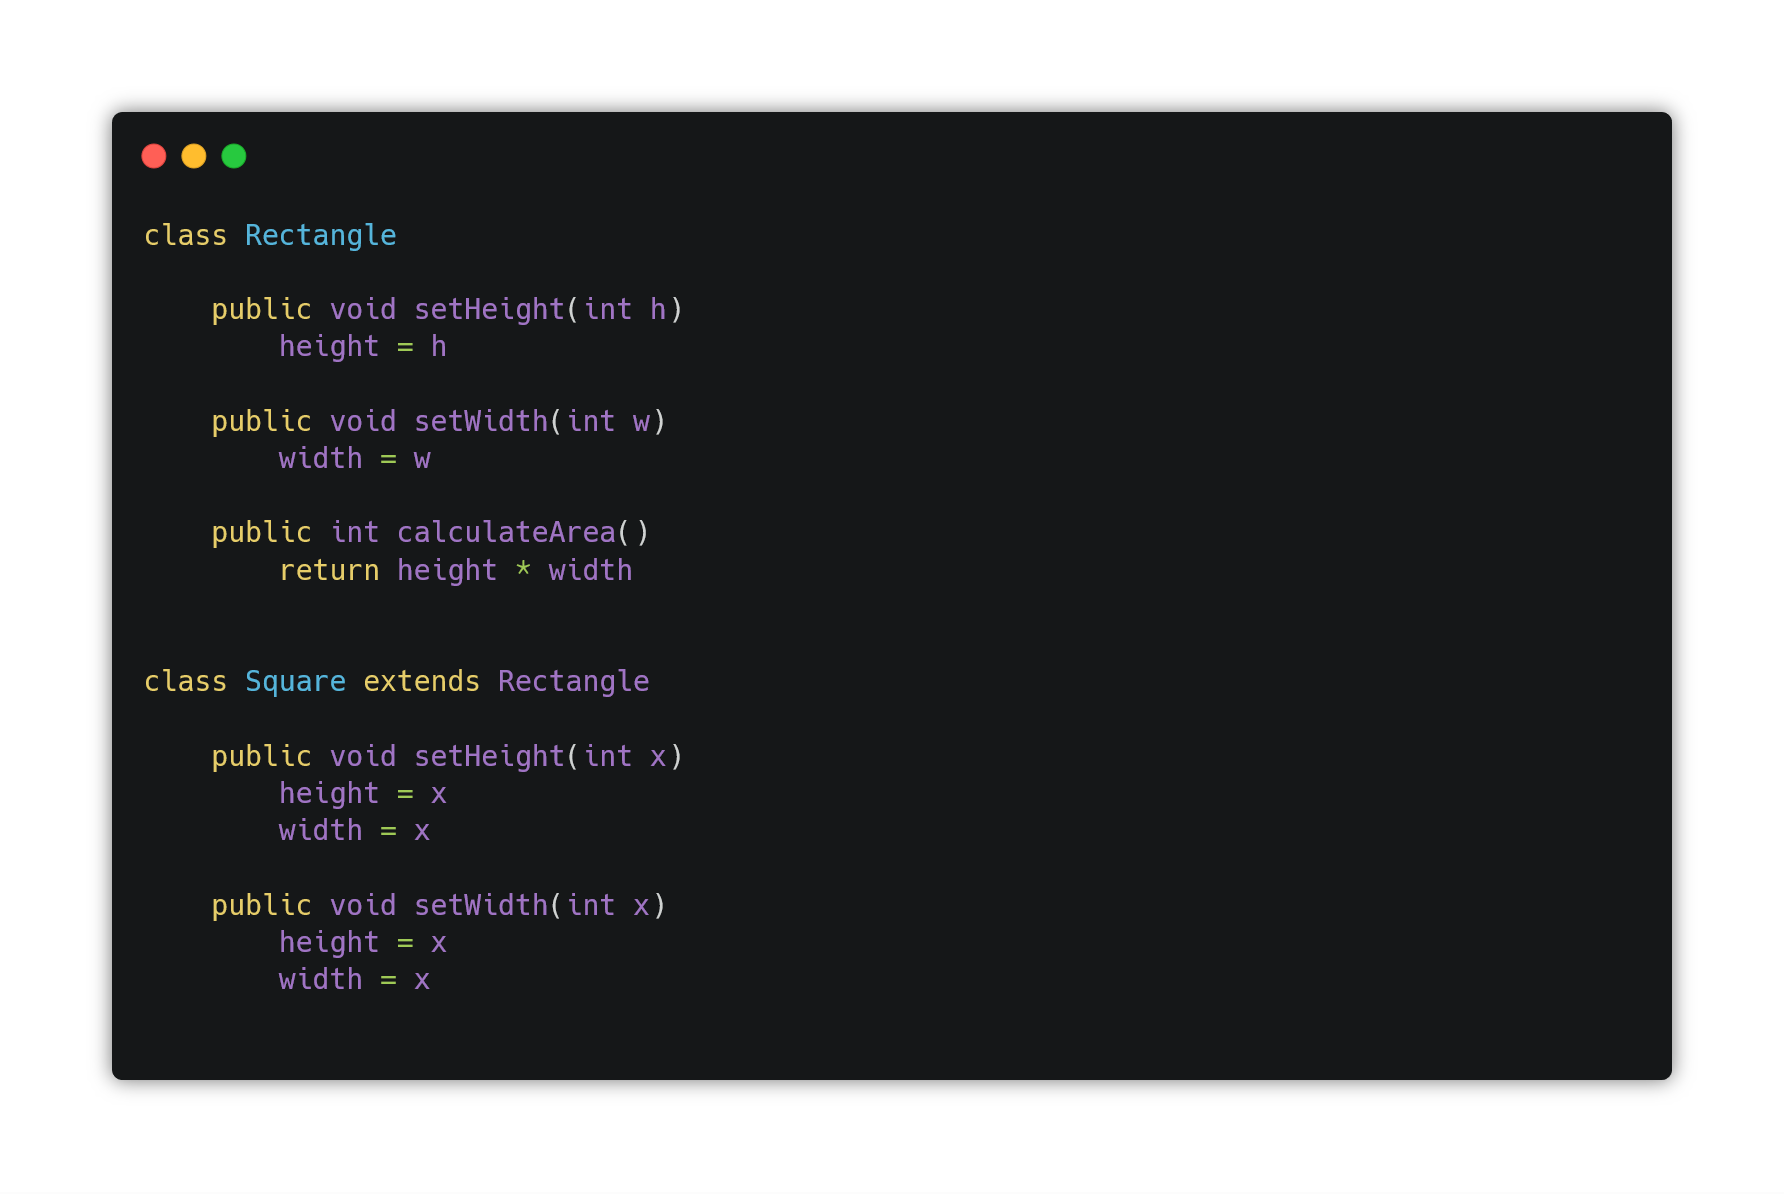
\includegraphics[width=\textwidth]{geometry.png}
	\end{figure}
\end{frame}

\begin{frame}{Zasada podstawienia Liskov}
	Każdy kwadrat jest prostokątem, jasna rzecz.
	
	Problem pojawi się jednak w miejscu, gdy \emph{podstawimy} obiekt klasy \texttt{Square} pod miejsce \texttt{Rectangle}. Pierwszy dziedziczy po drugim, więc powinny zachowywać się tak samo. Ale czy naprawdę się tak zachowują?
\end{frame}

\begin{frame}{Zasada podstawienia Liskov (ałć!)}
	\begin{figure} \centering
		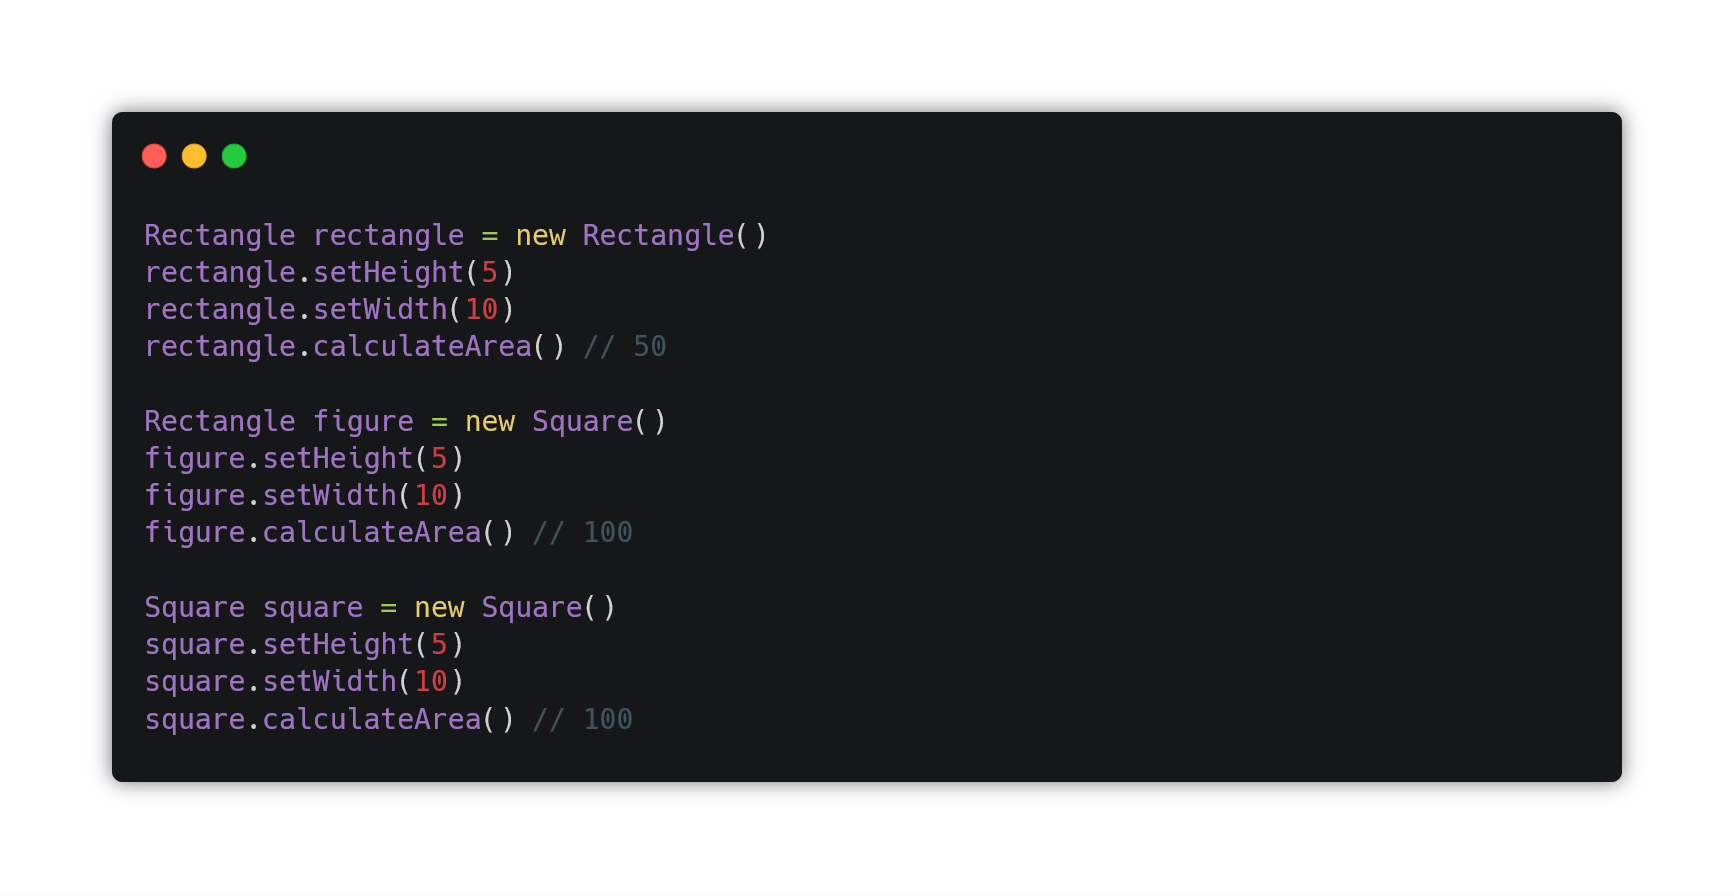
\includegraphics[width=\textwidth]{geometry2.png}
	\end{figure}
\end{frame}

\begin{frame}{Zasada podstawienia Liskov}
	Oczywiście w językach takich jak C++ można wykorzystać modyfikatory \texttt{virtual}, aby panować nad sytuacjami tego rodzaju, aczkolwiek sam kod wciąż będzie pogwałceniem zasady podstawienia Liskov.
\end{frame}

\section{I}

\begin{frame}{Zasada segregacji interfejsów}
	\textbf{I} (lub \textbf{ISP}) to \emph{interface segregation principle}, czyli zasada segregacji interfejsów.
\end{frame}

\begin{frame}{Zasada segregacji interfejsów}
	Programiści często sami dochodzą do stiwrdzenia jakoby wiele dedykowanych interfejsów jest lepszych niż jeden ogólny.
\end{frame}

\begin{frame}{Zasada segregacji interfejsów (ałć!)}
	\begin{figure} \centering
		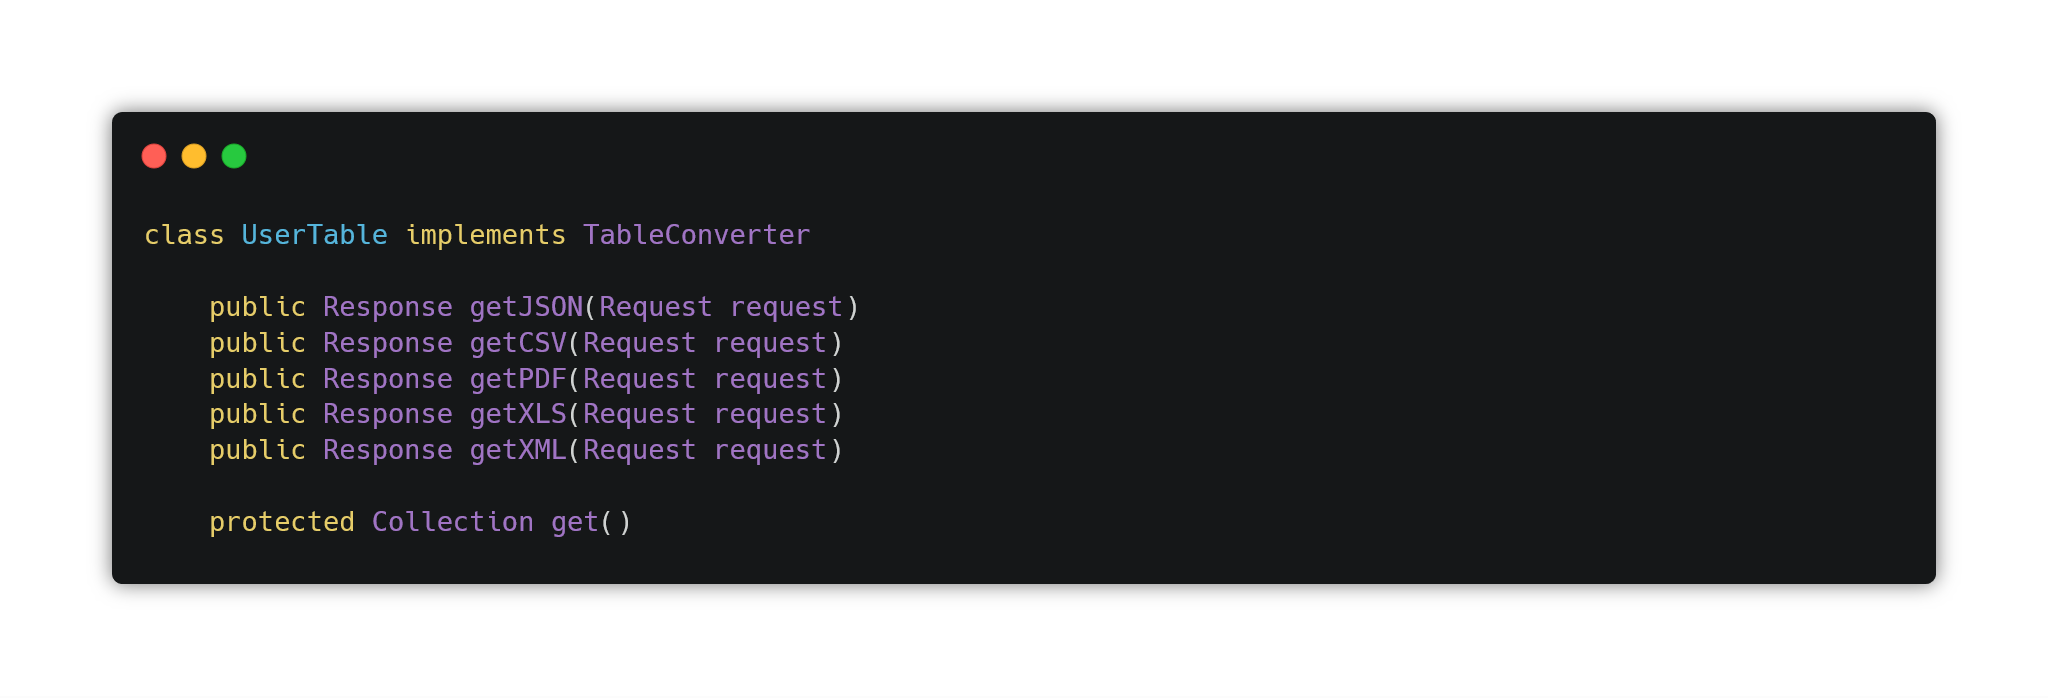
\includegraphics[width=\textwidth]{interfaces.png}
	\end{figure}
\end{frame}

\begin{frame}{Zasada segregacji interfejsów}
	A może lepiej byłoby to rozbić?
\end{frame}

\begin{frame}{Zasada segregacji interfejsów}
	\begin{figure} \centering
		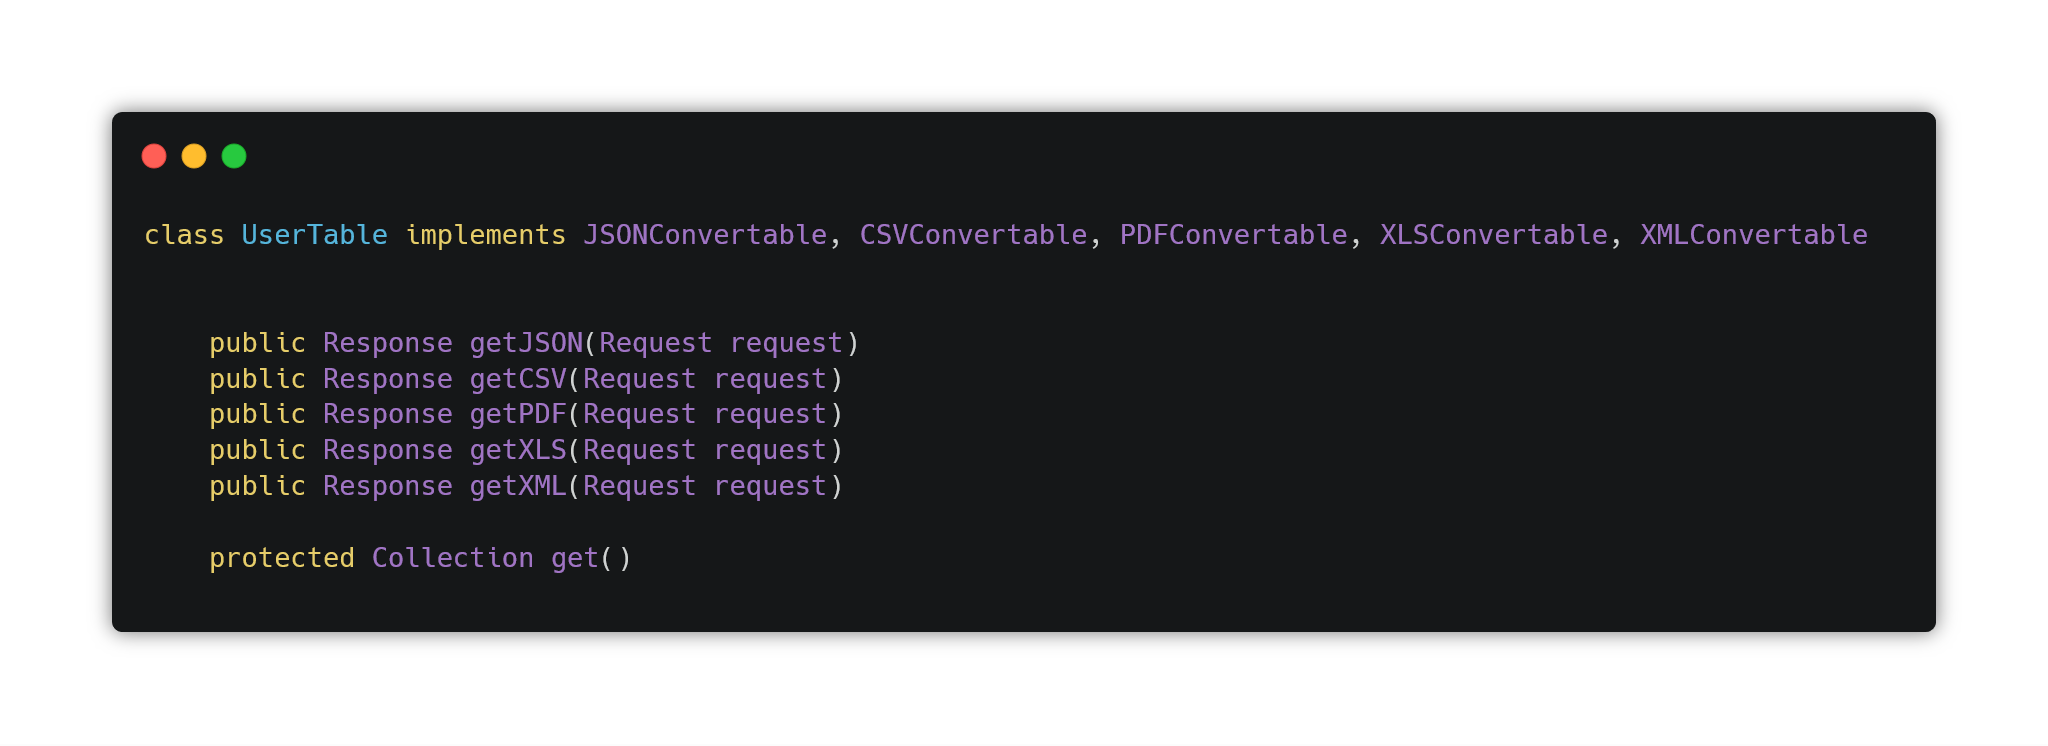
\includegraphics[width=\textwidth]{interfaces2.png}
	\end{figure}
\end{frame}

\begin{frame}{Zasada segregacji interfejsów}
	Warto pamiętać o dwóch rzeczach przy korzystaniu z interfejsów.
\end{frame}

\begin{frame}{Zasada segregacji interfejsów}
	Po pierwsze, interfejsy można po sobie dziedziczyć wielokrotnie (również w językach w których nie występuje wielodziedziczenia).
\end{frame}

\begin{frame}{Zasada segregacji interfejsów}
	Po drugie, interfejsy mogą być puste.
\end{frame}

\begin{frame}{Zasada segregacji interfejsów}
	Szybko się okaże, że ISP łączy się z SRP. 
\end{frame}

\begin{frame}{Zasada segregacji interfejsów}
	Zgodnie z zasadą lepiej mieć wiele krótkich interfejsów niż jeden wielki. Ale czy klasa z kilkoma interfejsami nie przeczy SRP?
\end{frame}

\section{D}

\begin{frame}{Zasada odwrócenia zależności}
	\textbf{D} (lub \textbf{DIP}) to \emph{dependency inversion principle}, czyli zasada odwrócenia zależności.
\end{frame}

\begin{frame}{Zasada odwrócenia zależności}
	\emph{Wysokopoziomowe moduły nie powinny zależeć od modułów niskopoziomowych.}
	
	\emph{Zależności między nimi powinny wynikać z abstrakcji.}
\end{frame}

\begin{frame}{Zasada odwrócenia zależności}
	To jest oczywiście rzecz, o której na wykładach mówiliśmy wielokrotnie.
\end{frame}

\begin{frame}{Zasada odwrócenia zależności}
	Wyobraźmy sobie serwis wielokrotnego użytku rejestrujący użytkowników. Wykorzystajmy klasę \texttt{User} dziedzicząca po modelu z ORM-a typu \emph{active record}.
	
	Taki serwis może być wykorzystany w wystawionym publicznie kontrolerze rejestracji, w panelu administracyjnym, z poziomu konsoli, a i pewnie też w wielu innych miejscach.
\end{frame}

\begin{frame}{Zasada odwrócenia zależności}
	\begin{figure} \centering
		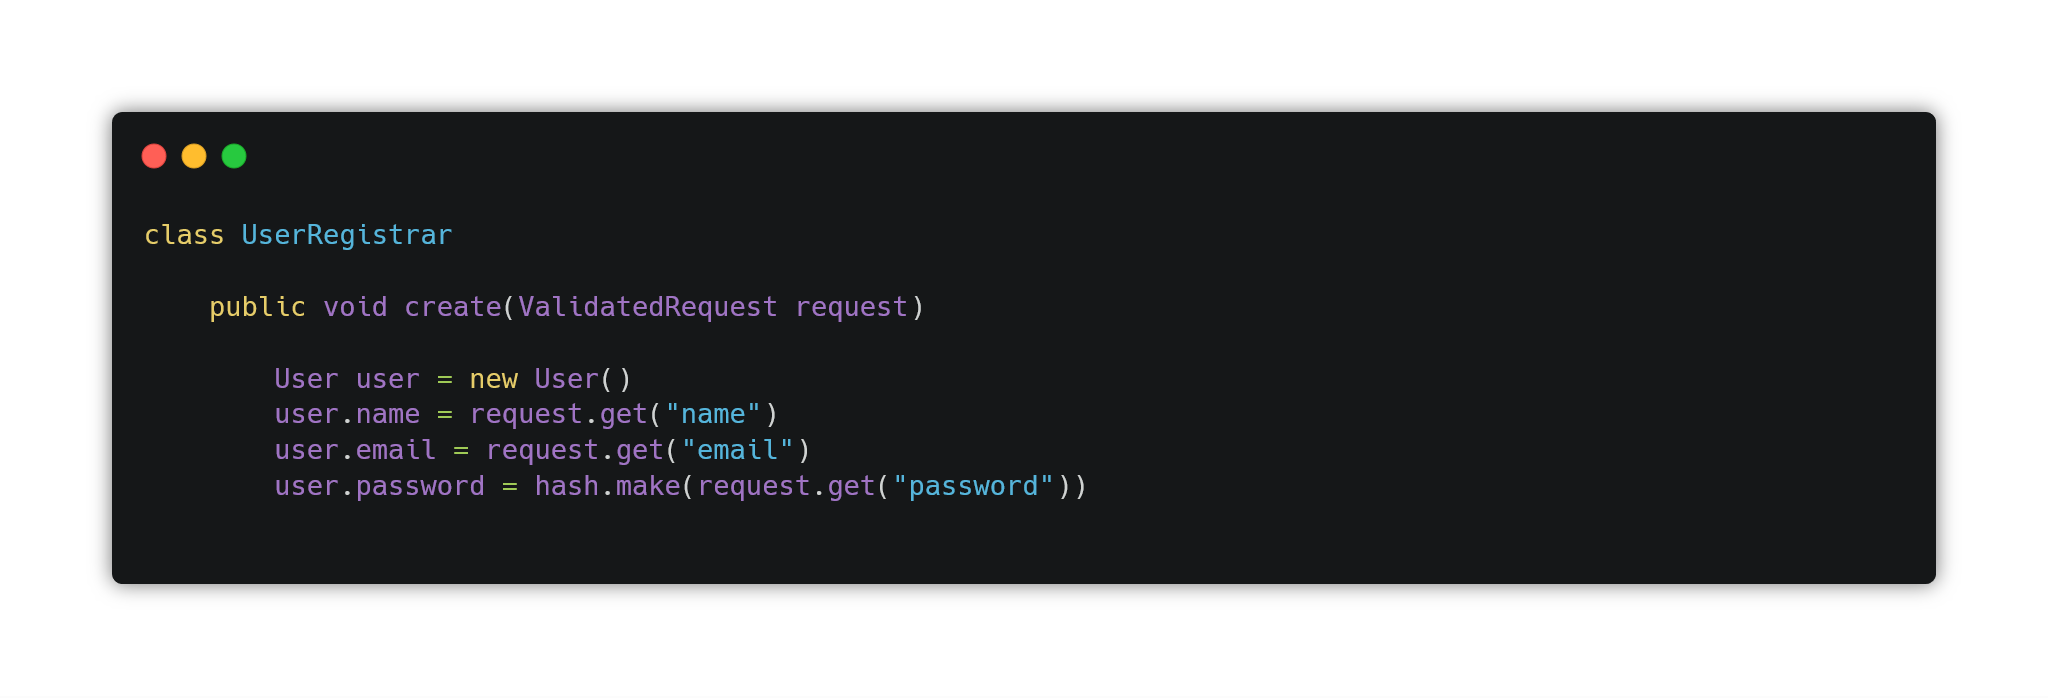
\includegraphics[width=\textwidth]{di.png}
	\end{figure}
\end{frame}

\begin{frame}{Zasada odwrócenia zależności}
	Łatwizna.
	
	A co jeżeli będziemy mieli osobny model administratora? Zaczyna się robic problem?
\end{frame}

\begin{frame}{Zasada odwrócenia zależności (ałć!)}
	\begin{figure} \centering
		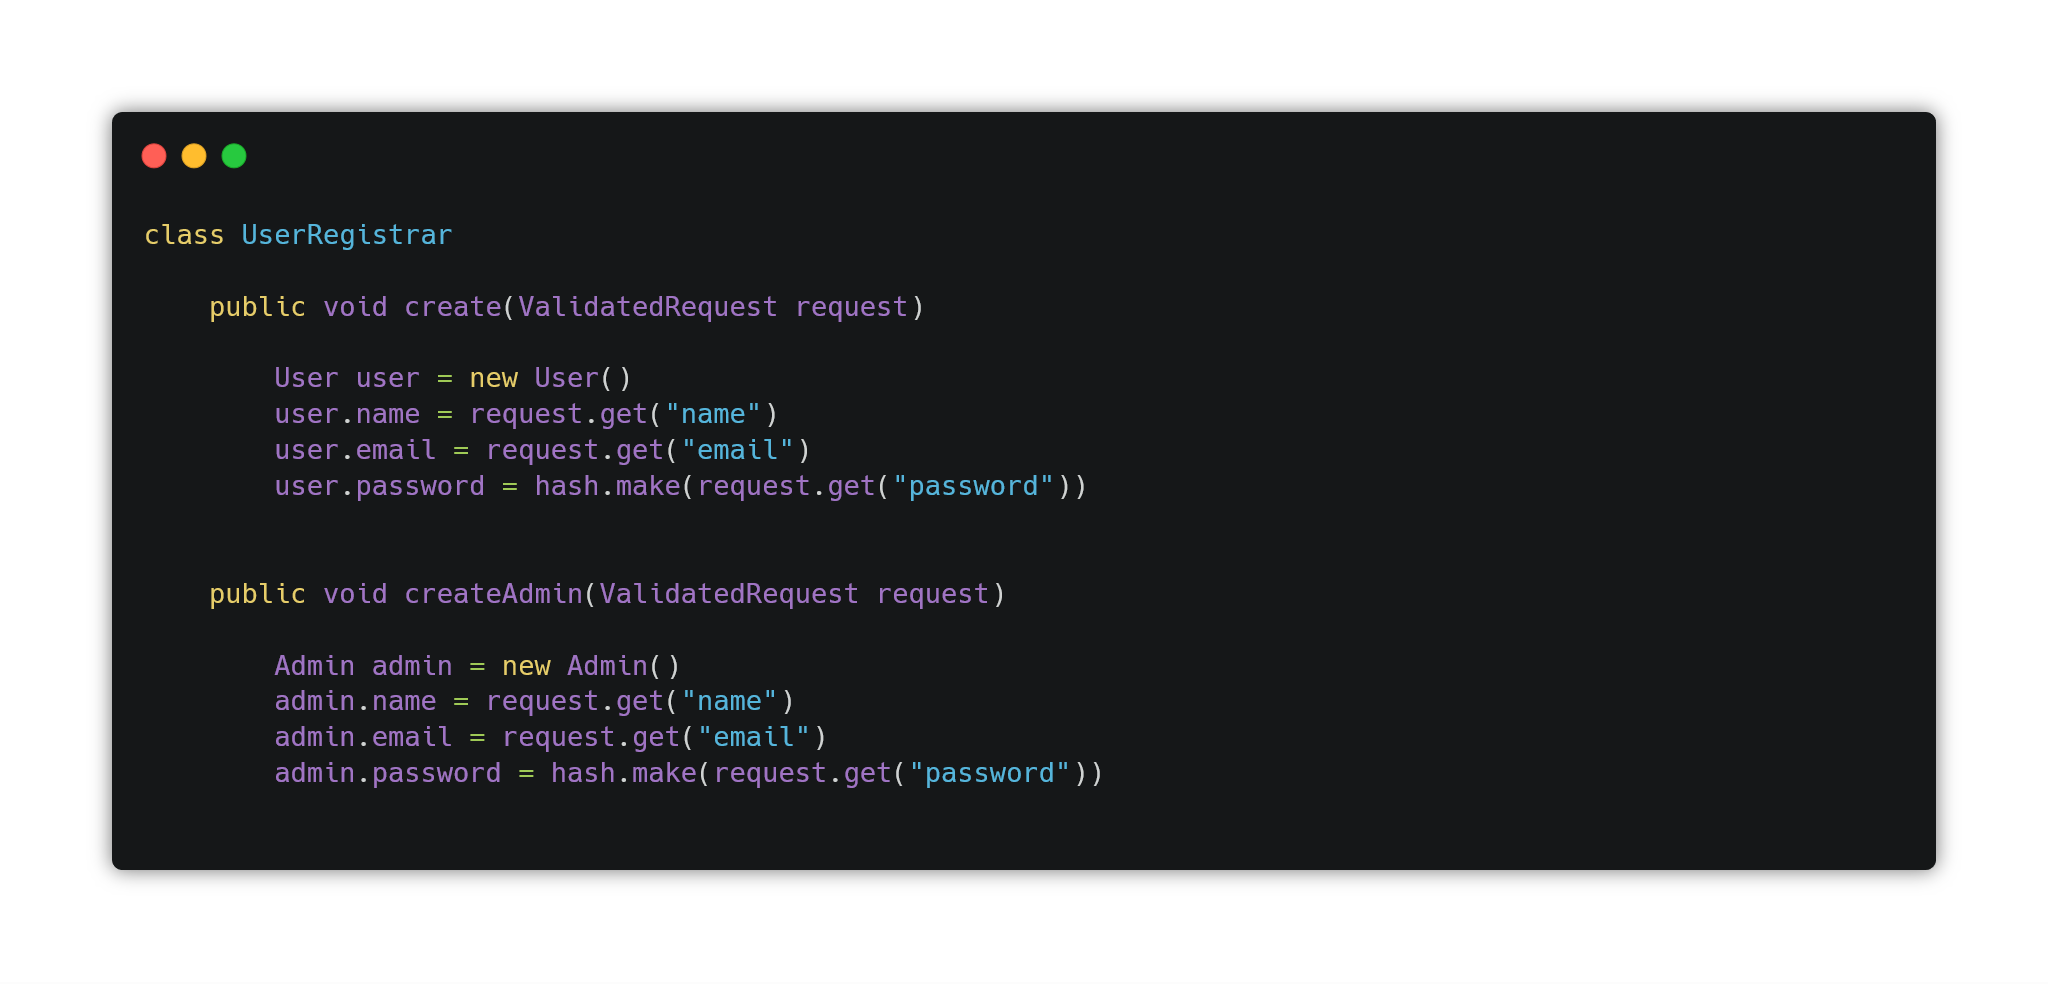
\includegraphics[width=\textwidth]{di2.png}
	\end{figure}
\end{frame}

\begin{frame}{Zasada odwrócenia zależności}
	Za dużo kodu się potwarza, wię może wypadałoby przesunąć część linijek do osobnej metody?
\end{frame}

\begin{frame}{Zasada odwrócenia zależności (ałć!)}
	\begin{figure} \centering
		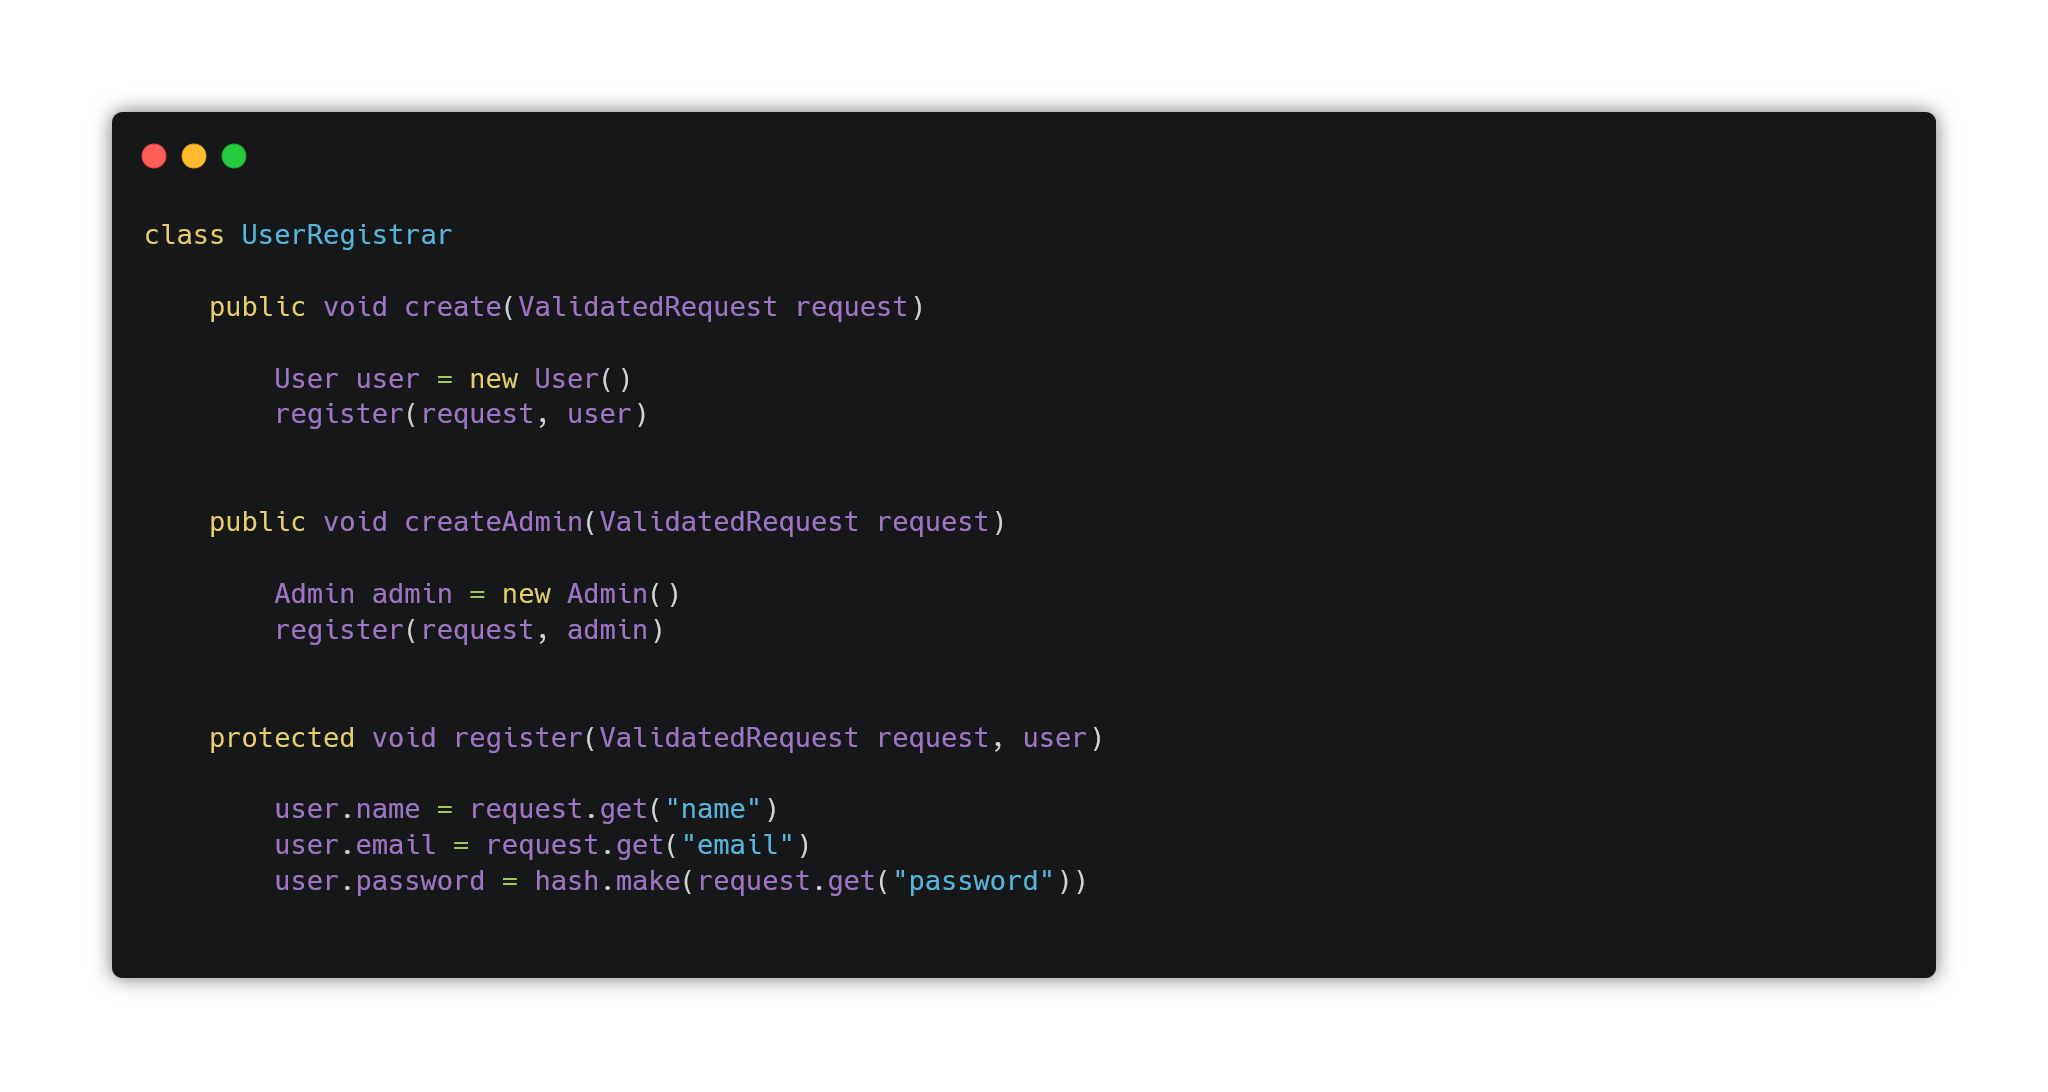
\includegraphics[width=\textwidth]{di3.png}
	\end{figure}
\end{frame}

\begin{frame}{Zasada odwrócenia zależności}
	W PHP czy Pythonie nie było problemu (w zależności oczywiście od ludzi robiących \emph{code review}). Ale i tak wypadałoby określić jakiś typ łączący użytkownika i administratora.
	
	Lepiej byłoby założyć, że jedno nie dziedziczy po drugim... na wszelki wypadek, gdyby zaraz miało pojawić się coś nowego.
\end{frame}

\begin{frame}{Zasada odwrócenia zależności (ałć!)}
	\begin{figure} \centering
		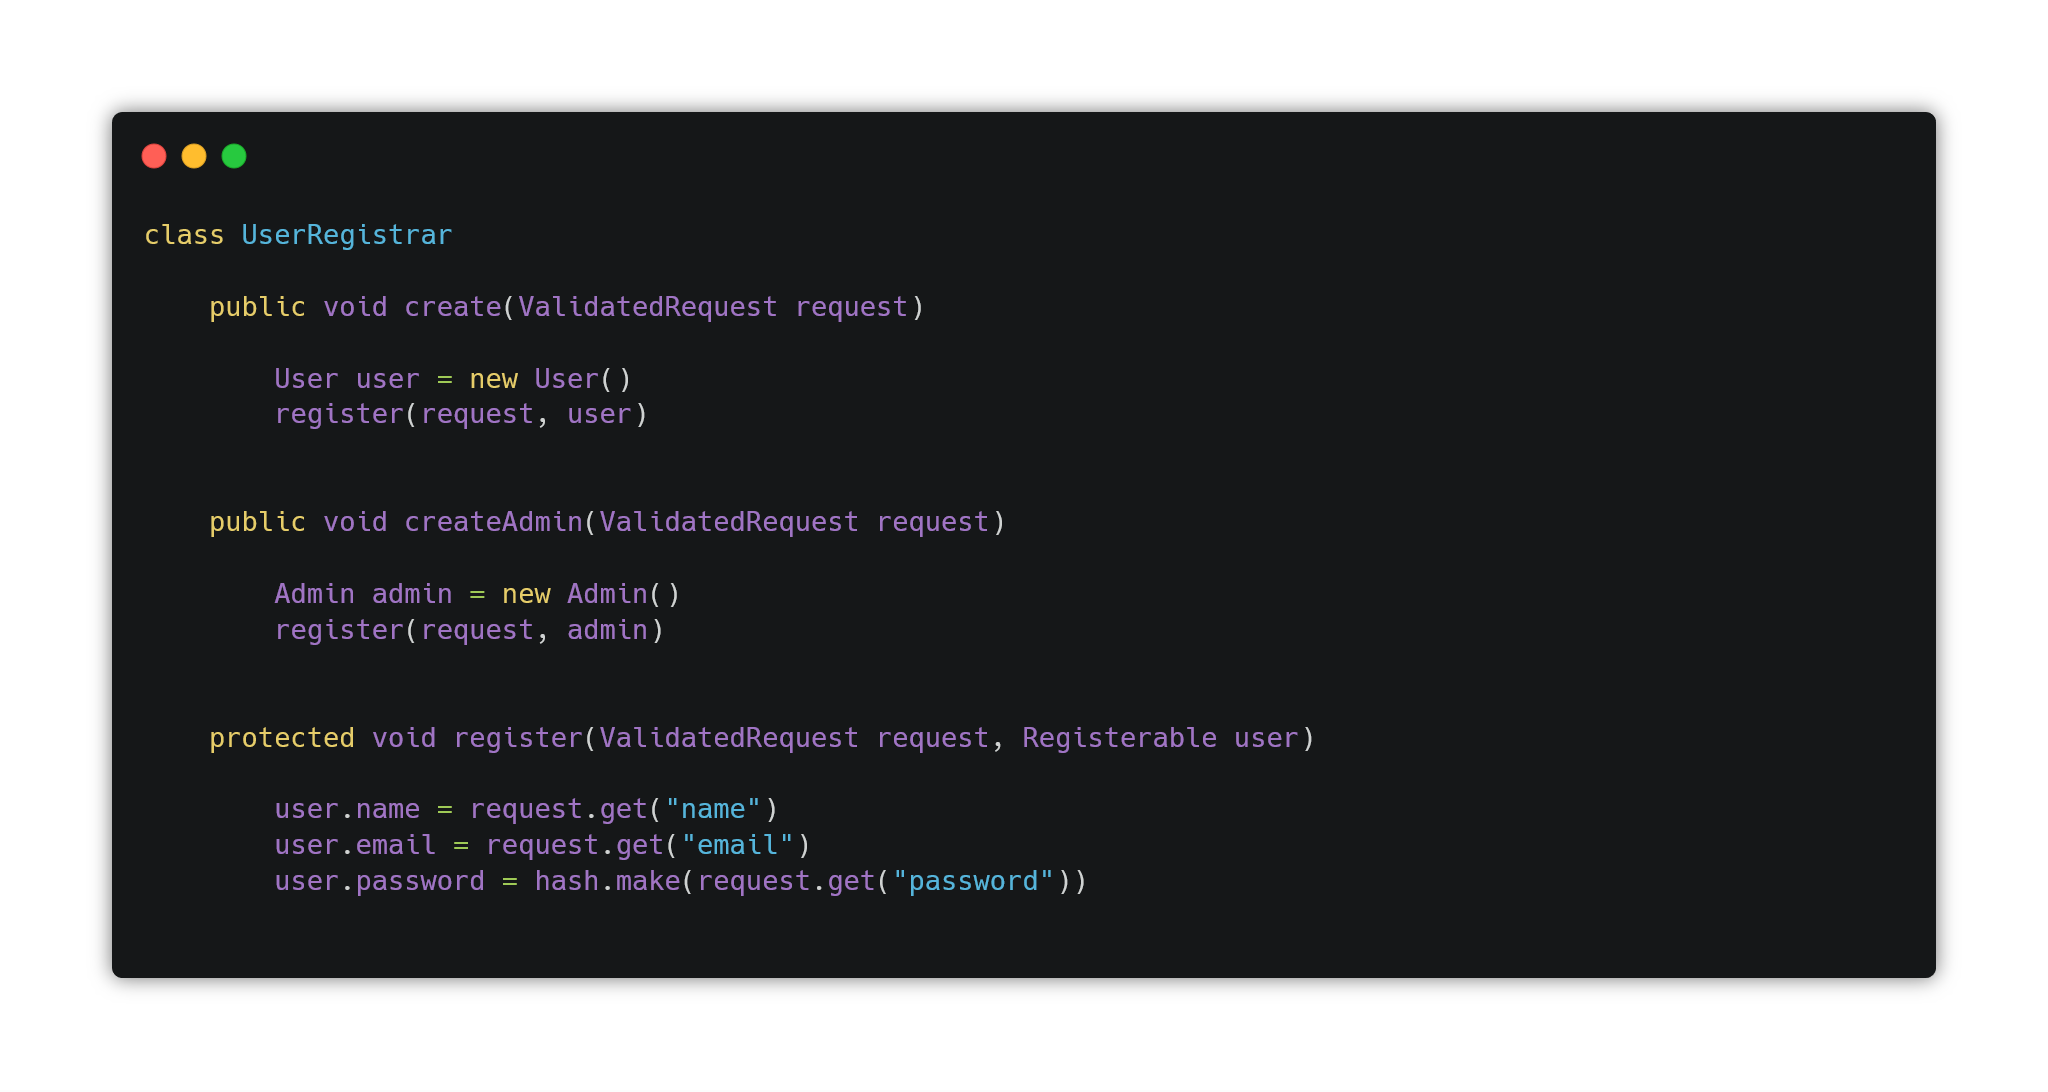
\includegraphics[width=\textwidth]{di4.png}
	\end{figure}
\end{frame}

\begin{frame}{Zasada odwrócenia zależności}
	I co? Okazuje się, że zbudowaliśmy podręcznikowy przykład implementacji wzorca odwrócenia sterowania w postaci wstrzykiwania zależności.
\end{frame}

\begin{frame}{Zasada odwrócenia zależności}
	\begin{figure} \centering
		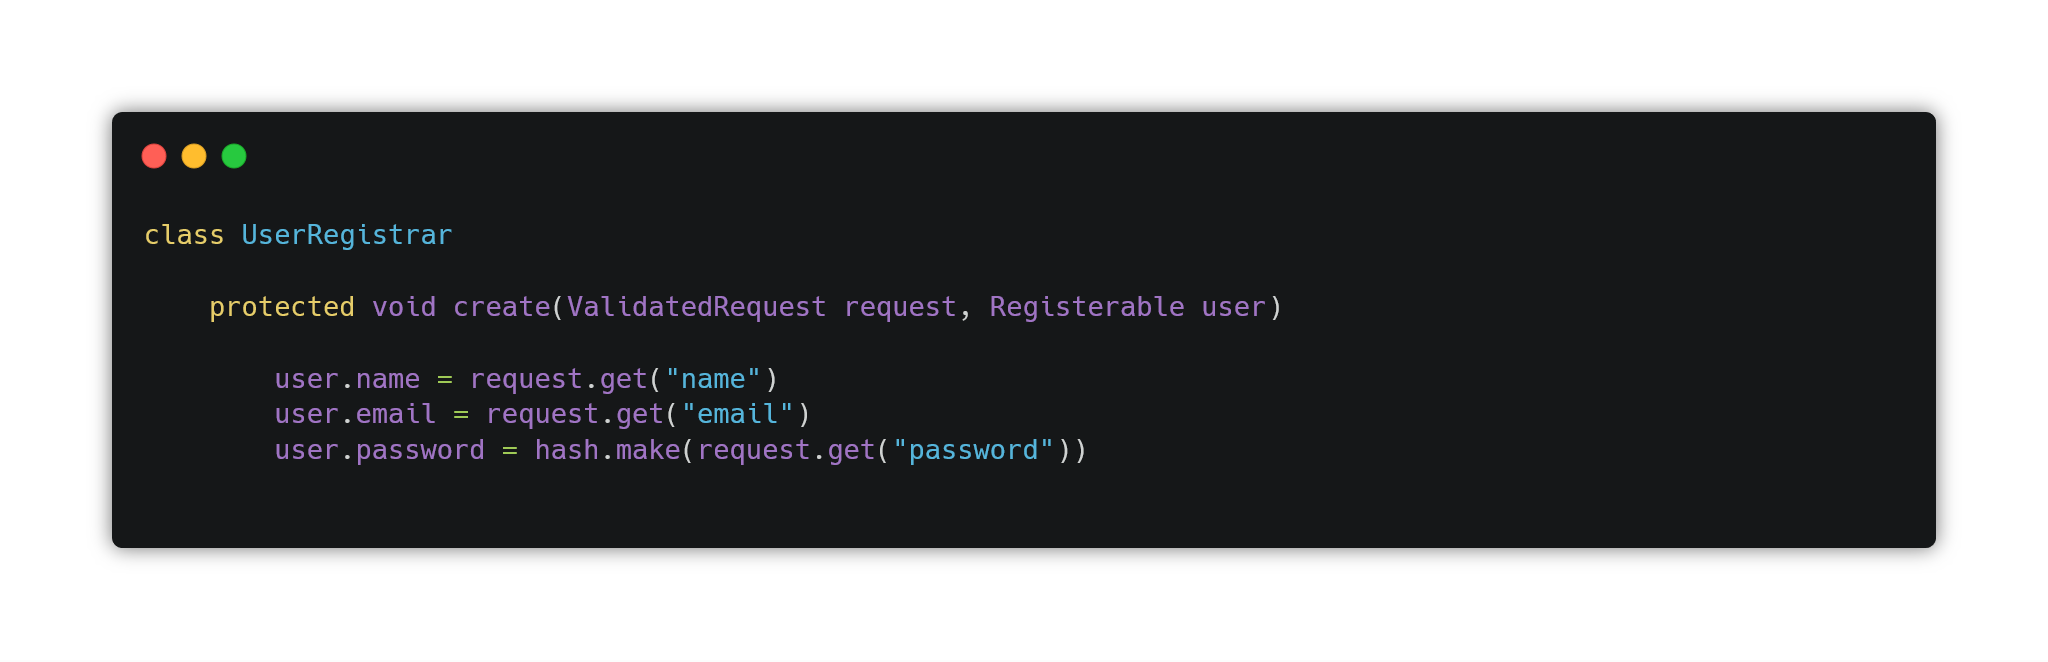
\includegraphics[width=\textwidth]{di5.png}
	\end{figure}
\end{frame}

\section{Podsumowanie}

\appendix

\begin{frame}[standout]
	Pytania?
\end{frame}

\begin{frame}{}

	Kod prezentacji dostępny jest w repozytorium git pod adresem \texttt{https://bitbucket.org/krewak/pwsz-ppsi} \\ \ \\

	\begin{figure}
		\centering
		\href{https://bitbucket.org/krewak/pwsz-ppsi}{
			
\includegraphics[width=.15\textwidth]{../_template/bitbucket.png}
		}
	\end{figure}
	
	Wszystkie informacje dot. kursu dostępne są pod adresem \texttt{http://pwsz.rewak.pl/kursy/4} \\ \ \\

	\begin{figure}
		\centering
		\href{http://pwsz.rewak.pl/kursy/3}{
			
\includegraphics[width=.15\textwidth]{../_template/rewak.png}
		}
	\end{figure}

\end{frame}

\end{document}
